\section{ĐƠN VỊ VÀ SAI SỐ TRONG VẬT LÍ}
\subsection{LÝ THUYẾT TRỌNG TÂM}
\begin{tomtat}
	\subsubsection{Đơn vị và thứ nguyên trong vật lí}
	\paragraph{Hệ đơn vị SI, đơn vị cơ bản và đơn vị dẫn xuất}
	\begin{dn}
		Tập hợp của đơn vị được gọi là hệ đơn vị. Trong khoa học có rất nhiều hệ đơn vị được sử dụng, trong đó thông dụng nhất là hệ đơn vị đo lường quốc tế SI (Système International d’unités) được xây dựng trên cơ sở của \textbf{7 đơn vị cơ bản}.
	\end{dn}
\begin{center}
	\captionof{table}{Các đơn vị cơ bản trong hệ SI}
	\begin{tabular}{|c|c|c|c|}
		\hline
		\thead{STT} & \thead{Đơn vị} & \thead{Kí hiệu} & \thead{Đại lượng}\\
		\hline
		$1$ & \text{mét} & $\si{\meter}$ & \text{Chiều dài}\\
		\hline
		$2$ & \text{kilôgam} & $\si{\kilo\gram}$ & \text{Khối lượng}\\
		\hline
		$3$ & \text{giây} & $\si{\second}$ & \text{Thời gian}\\
		\hline
		$4$ & \text{kelvin} & $\si{\kelvin}$ & \text{Nhiệt độ}\\
		\hline
		$5$ & \text{ampe}& $\si{\ampere}$ & \text{Cường độ dòng điện}\\ 
		\hline
		$6$ & \text{mol} & $\si{\mole}$ & \text{Lượng chất}\\
		\hline
		$7$ & \text{candela} & $\si{\candela}$ & \text{Cường độ sáng}\\
		\hline
	\end{tabular}
\end{center}
\begin{dn}
	\textbf{Đơn vị dẫn xuất:} Ngoài 7 đơn vị cơ bản, những đơn vị còn lại được gọi là đơn vị dẫn xuất. \\Mọi đơn vị dẫn xuất đều có thể phân tích thành các đơn vị cơ bản dựa vào mối liên hệ giữa các đại lượng tương ứng.
\end{dn}
\paragraph{Thứ nguyên}
Thứ nguyên của một đại lượng là quy luật nêu lên sự phụ thuộc của đơn vị đo đại lượng đó vào các đơn vị cơ bản.
\begin{itemize}
	\item Thứ nguyên của một đại lượng $X$ được biễn diễn dưới dạng $[X]$. Thứ nguyên của một số đại lượng cơ bản thường sử dụng được thể hiện trong Bảng \ref{tab:2}.
	\item Một đại lượng vật lí có thể được biểu diễn bằng nhiều đơn vị khác nhau nhưng chỉ có một thứ nguyên duy nhất. Một số đại lượng vật lí có thể có cùng thứ nguyên.
\end{itemize}
\begin{center}
	\captionof{table}{Thứ nguyên của một số đại lượng cơ bản}
	\label{tab:2}
	\begin{tabular}{|c|c|}
		\hline
		\thead{Đại lượng cơ bản} & \thead{Thứ nguyên}\\
		\hline
		\text{[Chiều dài]} & $L$\\
		\hline
		\text{[Khối lượng]} & $M$\\
		\hline
		\text{[Thời gian]} & $T$\\
		\hline
		\text{[Cường độ dòng điện]} & $I$\\
		\hline
		\text{[Nhiệt độ]} & $K$\\
		\hline
	\end{tabular}
\end{center}
\begin{luuy}
	Trong các biểu thức vật lí:
	\begin{itemize}
		\item Các số hạng trong phép cộng (hoặc trừ) phải có cùng thứ nguyên.
		\item Hai vế của một biểu thức vật lí có cùng thứ nguyên.
	\end{itemize}
\end{luuy}
\paragraph{Tên và kí hiệu các tiếp đầu ngữ của bội số, ước số thập phân của đơn vị}
	Khi số đo của đại lượng đang xem xét là một bội số hoặc ước số thập phân của mười, ta có thể sử dụng tiếp đầu ngữ như trong Bảng \ref{tab:1} ngay trước đơn vị để phần số đo được trình bày ngắn gọn.
	\begin{center}
		\captionof{table}{Tên và kí hiệu tiếp đầu ngữ của bội số, ước số thập phân của đơn vị}
		\begin{tabular}{|c|c|c|c|c|c|}
			\hline
			\thead{Kí hiệu} & \thead{Tên đọc} & \thead{Hệ số} & \thead{Kí hiệu} & \thead{Tên đọc} & \thead{Hệ số}\\
			\hline
			Y & \text{yotta} & $10^{24}$ & \text{y} & \text{yokto} & $10^{-24}$\\
			\hline
			Z & \text{zetta} & $10^{21}$ & z & \text{zepto} & $10^{-21}$\\
			\hline
			E & \text{eta} & $10^{18}$ & \text{a} & \text{atto} & $10^{-18}$\\
			\hline
			P & \text{peta} & $10^{15}$ & f & \text{femto} & $10^{-15}$\\
			\hline
			T & \text{tera} & $10^{12}$ & p & \text{pico} & $10^{-12}$\\
			\hline
			G & \text{giga} & $10^{9}$ & n & \text{nano} & $10^{-9}$\\
			\hline
			M & \text{mega} & $10^{6}$ & \text{$\mu$} & \text{micro} & $10^{-6}$\\
			\hline
			k & \text{kilo} & $10^{3}$ & m & \text{mili} & $10^{-3}$\\
			\hline
			h & \text{hecto} & $10^{2}$ & c & \text{centi} & $10^{-2}$\\
			\hline
			da & \text{deka} & $10^{1}$ & d & \text{deci} & $10^{-1}$\\
			\hline
		\end{tabular}
		\label{tab:1}
	\end{center}
	
	\subsubsection{Sai số trong phép đo và cách hạn chế}
	\paragraph{Phép đo các đại lượng vật lí}
	Phép đo một đại lượng vật lí là phép so sánh nó với đại lượng cùng loại được quy ước làm đơn vị.\\	
	Phép đo được phân loại thành 
	\begin{itemize}
		\item \textbf{Phép đo trực tiếp} là phép xác định giá trị  một đại lượng bằng cách so sánh trực tiếp với dụng cụ đo (ví dụ như đo khối lượng bằng cân, đo nhiệt độ bằng nhiệt kế). 
		\item \textbf{Phép đo gián tiếp} là phép xác định giá trị một đại lượng thông qua một công thức liên hệ với các đại lượng được đo trực tiếp (ví dụ như đo khối lượng riêng thông qua việc xác định khối lượng và thể tích của khối vật chất).   
	\end{itemize}
	\paragraph{Các loại sai số của phép đo}
	\begin{center}
		\captionof{table}{Các loại sai số của phép đo}
		\begin{longtable}{|m{5em}|m{7.5cm}|m{7.5cm}|}
			\hline
			&\thead{Sai số hệ thống} & \thead{Sai số ngẫu nhiên}\\
			\hline
			\thead{Khái\\ niệm} & Sai số hệ thống là sai số có tính quy luật và được lặp lại ở tất cả các lần đo. Sai số hệ thống làm cho giá trị đo tăng hoặc giảm một lượng nhất định so với giá trị thực. & Sai số ngẫu nhiên là sai số xuất phát từ sai sót, phản xạ của người làm thí nghiệm hoặc từ những yếu tố ngẫu nhiên bên ngoài.\\
			\hline
			\thead{Nguyên\\ nhân} & Các dụng cụ đo các đại lượng vật lí luôn có sự sai lệch do đặc điểm và cấu tạo của dụng cụ gây ra. & Sai số này thường có nguyên nhân không rõ ràng và dẫn đến sự phân tán của các kết quả đo xung quanh một giá trị trung bình.\\
			\hline
			\thead{Cách\\ hạn chế} & Sai số hệ thống có thể được hạn chế bằng cách thường xuyên hiệu chỉnh dụng cụ đo, sử dụng thiết bị đo có độ chính xác cao. & Sai số ngẫu nhiên có thể được hạn chế bằng cách thực hiện phép đo nhiều lần và lấy giá trị trung bình để hạn chế sự phân tán của số liệu đo.\\
			\hline
		\end{longtable}
	\end{center}
	\begin{luuy}
		Đối với một số dụng cụ đo, sai số dụng cụ thường được xác định bằng một nửa độ chia nhỏ nhất.
	\end{luuy}
	\subsubsection{Biểu diễn kết quả đo}
	\paragraph{Cách biểu diễn sai số của phép đo}
	Khi đo $n$ lần cùng một đại lượng $A$, ta thu được các giá trị khác nhau: $A_1,\, A_2,\,...,A_n$\\
	Giá trị trung bình khi đo nhiều lần một đại lượng $A$:$$\bar{A}=\dfrac{A_1+A_2+...+A_{\text{n}}}{n},$$
	là giá trị gần đúng nhất với giá trị thực của đại lượng $A$.  
	\begin{itemize}
		\item Sai số tuyệt đối ứng với mỗi lần đo:
		$$\Delta A_1=|\bar{A}-A_1|;\quad\Delta A_2=|\bar{A}-A_2|;\quad\Delta A_3=|\bar{A}-A_3|;\dots; \Delta A_i=\left|\overline{A}-A_i\right|$$
		\item Sai số ngẫu nhiên là sai số tuyệt đối trung bình của $n$ lần đo:
		$$\overline{\Delta A}=\dfrac{\Delta A_1+\Delta A_2+...+\Delta A_{\textrm{n}} }{n}.$$
		\item Sai số dụng cụ $\Delta A_\text{dc}$ thường được lấy bằng nửa độ chia nhỏ nhất đối với những dụng cụ đơn giản như thước kẻ, cân bàn, bình chia độ, \dots Trong nhiều trường hợp, sai số dụng cụ thường được cung cấp chính xác bởi nhà sản xuất.
		\item Sai số tuyệt đối của phép đo cho biết phạm vi biến thiên của giá trị đo được và bằng tổng của sai số ngẫu nhiên và sai số dụng cụ:
		$$\Delta A= \overline{\Delta A}+ \Delta A_\text{dc}.$$
	\end{itemize}
	\paragraph{Sai số tương đối (tỉ đối)}
	Sai số tỉ đối $\delta A$ của phép đo là tỉ số giữa \textbf{sai số tuyệt đối} và \textbf{giá trị trung bình} của đại lượng cần đo, tính bằng phần trăm:
	$$\delta A=\dfrac{\Delta A}{\overline A}\cdot 100\%.$$
	Sai số tỉ đối càng \textbf{nhỏ} thì phép đo càng chính xác.
	\paragraph{Cách xác định sai số của phép đo gián tiếp}
	Sai số của phép đo gián tiếp, được xác định theo các quy tắc:
	\begin{itemize}
		\item Sai số tuyệt đối của một tổng hay hiệu thì bằng \textbf{tổng} các sai số tuyệt đối của các số hạng:\\
		Nếu $F=x\pm y\pm z \dots$ thì $\Delta F = \Delta x + \Delta y + \Delta z+\dots$.
		\item Sai số tỉ đối của một tích hay thương thì bằng \textbf{tổng} các sai số tỉ đối của các thừa số:\\ 
		Nếu $F= x^m\cdot\dfrac{y^n}{z^k}$ thì $\delta F=m\cdot\delta x+n\cdot\delta y +k\cdot\delta z$.
	\end{itemize}
	\begin{noidung}{Quy tắc xác định số chữ số có nghĩa (CSCN):}
			Các chữ số có nghĩa bao gồm:
		\begin{itemize}
			\item Các chữ số khác 0.
			\item Các chữ số 0 nằm giữa hai chữ số khác 0.
			\item Các chữ số 0 nằm bên phải của dấu	thập phân và một chữ số khác 0
		\end{itemize}
	\end{noidung}
	\textit{Ví dụ:} \textbf{678} có ba chữ số có nghĩa, \textbf{6008} có bốn chữ số có nghĩa, 0,0\textbf{800} có ba chữ số có nghĩa.
	\paragraph{Cách viết kết quả đo}
	$$A=\overline{A} \pm \Delta A,$$
	trong đó:
	\begin{itemize}
		\item $\overline A$ là giá trị trung bình,
		\item $\Delta A$ là sai số tuyệt đối. 
	\end{itemize}
\end{tomtat}
\subsection{VÍ DỤ MINH HỌA}
\begin{dang}{Tìm hiểu một số loại sai số đơn giản hay gặp khi đo các đại lượng vật lí và cách khắc phục chúng}
	\end{dang}
	\begin{vd}
		Quan sát các hình sau và phân tích các nguyên nhân gây ra sai số của phép đo trong các trường hợp được nêu
		\begin{center}
			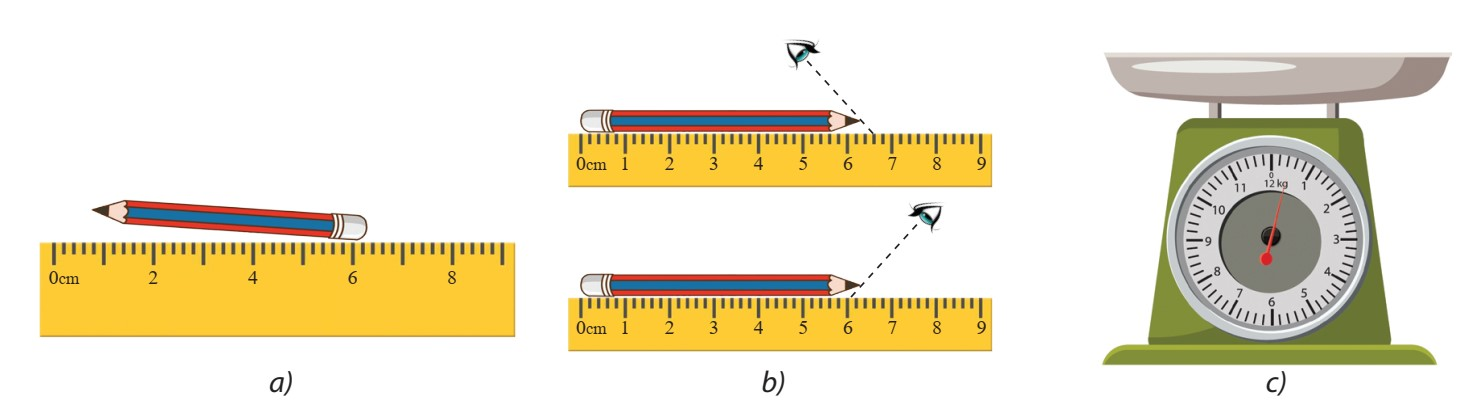
\includegraphics[scale=0.5]{figs/G10Y25B2-1}
		\end{center}
		\loigiai{
			\begin{enumerate}[label=\alph*)]
				\item Đặt bút không dọc theo thước, đầu bút không trùng với vạch số 0.
				\item Đặt mắt sai cách, hướng nhìn không vuông góc.
				\item Kim cân chưa được hiệu chỉnh về số 0.
			\end{enumerate}
		}
	\end{vd}
\begin{dang}{Vận dụng mối liên hệ giữa đơn vị dẫn xuất với 7 đơn vị cơ bản của hệ SI}
\end{dang}
\begin{vd}
	Để xác định quãng đường đi được $s$ của một chất điểm chuyển động thẳng đều, một bạn học sinh đã viết công thức như sau: $s=\alpha\cdot v\cdot t^2$ với $v$ và $t$ lần lượt là vận tốc và thời gian, $\alpha$ là hằng số không thứ nguyên. Dựa vào việc xác định thứ nguyên, em hãy cho biết công thức trên là đúng hay sai.
	\loigiai{
		Thứ nguyên của các đại lượng $s$, $v$ và $t$ lần lượt là
		\begin{itemize}
			\item $\left[s\right]=L$
			\item $\left[v\right]=L\cdot T^{-1}$
			\item $\left[t\right]=T$
		\end{itemize}
		Từ đó, ta thấy vế trái của công thức trên có thứ nguyên $L$ trong khi vế phải lại có thứ nguyên $L\cdot T$. Do 2 vế của công thức không cùng thứ nguyên nên bạn học sinh chưa đưa ra được công thức chính xác.
		Dựa vào phân tích thứ nguyên, ta cần sửa lại công thức chính xác như sau:
		$$s=\alpha \cdot v\cdot t$$
		Trong hệ SI, $s$, $v$ và $t$ lần lượt có đơn vị là $\si{\meter}, \si{\meter\cdot\second^{-1}}, \si{\second}$.
	}
\end{vd}
\begin{dang}{Xác định được sai số tuyệt đối, sai số tỉ đối và biểu diễn được kết quả đo}
\end{dang}
\begin{vd}
	Cho bảng số liệu thể hiện kết quả đo đường kính của một viên bi thép bằng thước kẹp có sai số dụng cụ là $\SI{0.02}{\milli\meter}$. Tính sai số tuyệt đối, sai số tương đối của phép đo và biểu diễn kết quả đo có kèm theo sai số
	\begin{longtable}{|c|c|c|}
		\hline
		\thead{Lần đo} & \thead{$d \left(\si{\milli\meter}\right)$} & \thead{$\Delta d \left(\si{\milli\meter}\right)$}\\
		\hline
		1 & 6,32 & \dots\\
		\hline
		2 & 6,32 & \dots\\
		\hline
		3 & 6,32 & \dots\\
		\hline
		4 & 6,32 & \dots\\
		\hline
		5 & 6,34 & \dots\\
		\hline
		6 & 6,34 & \dots\\
		\hline
		7 & 6,32 & \dots\\
		\hline
		8 & 6,34 & \dots\\
		\hline
		9 & 6,32 & \dots\\
		\hline
		\textbf{Trung bình} & $\overline{d}=?$ & $\overline{\Delta d}=?$\\
		\hline
	\end{longtable}
	
	\loigiai{
		Giá trị trung bình của đường kính viên bi:
		$$\overline{d}=\dfrac{d_1+d_2+d_3+\dots+d_9}{9}\approx\SI{6.327}{\milli\meter}$$
		Sai số tuyệt đối ứng với mỗi lần đo
		$$\Delta d_i=\left|\overline{d}-d_i\right|$$
		$$\Delta d_1=\Delta d_2=\Delta d_3=\Delta d_4=\Delta d_7=\Delta d_9=\left|\SI{6.327}{\milli\meter}-\SI{6.32}{\milli\meter}\right|=\SI{0.007}{\milli\meter}$$
		$$\Delta d_5=\Delta d_6=\Delta d_8=\left|\SI{6.327}{\milli\meter}-\SI{6.34}{\milli\meter}\right|=\SI{0.013}{\milli\meter}$$
		Sai số tuyệt đối trung bình của phép đo:
		$$\overline{\Delta d}=\dfrac{\Delta d_1+\Delta d_2+\dots+\Delta d_9}{9}=\SI{0.009}{\milli\meter}$$
		Sai số tuyệt đối của phép đo:
		$$\Delta d = \overline{\Delta d}+\Delta d_\text{dc}=\SI{0.009}{\milli\meter}+\SI{0.02}{\milli\meter}=\SI{0.029}{\milli\meter}$$
		Sai số tương đối của phép đo:
		$$\delta d =\dfrac{\Delta d}{\overline{d}}\cdot\SI{100}{\percent}\approx\SI{0.46}{\percent}$$
		Kết quả phép đo:
		$$d=\overline{d}\pm\Delta d=\SI{6.273}{\milli\meter}\pm\SI{0.029}{\milli\meter}.$$
	}
\end{vd}

\begin{vd}
	Trong bài thực hành đo gia tốc trọng trường của Trái Đất tại phòng thí nghiệm, một học sinh đo được chiều dài của con lắc đơn $\ell= \xsi{800\pm 1}{\milli\meter}$ thì chu kì dao động là $T = \xsi{1.78\pm 0.02}{\second}$. Lấy $\pi=\SI{3.14}{}$. Biết chu kỳ của con lắc đơn tính theo công thức $T=2\pi \sqrt{\dfrac{\ell}{g}}$. Gia tốc trọng trường $g$ của Trái Đái tại phòng thí nghiệm đó là bao nhiêu?
	\loigiai{
		Từ công thức: $$T=2\pi \sqrt{\dfrac{\ell}{g}} \Rightarrow g=\dfrac{4\pi^2\ell}{T^2}.$$ 	
		
		Giá trị trung bình của gia tốc trọng trường: 	
		$$\overline{g}=\dfrac{4\pi^2\ell}{T^2}=\dfrac{4\pi^2\cdot \SI{3.14}{}\cdot \SI{0.8}{\meter}}{\left( \SI{1.78}{\second}\right)^2}=\SI{9.96}{\meter\per\second^2}.$$
		
		Sai số tuyệt đối của gia tốc trọng trường:
		\begin{align*}
			\dfrac{\Delta g}{\overline g}&= \dfrac{\Delta \ell}{\overline \ell}+ 2\dfrac{\Delta T}{\overline T}\\
			&=\dfrac{\SI{1}{\milli\meter}}{\SI{800}{\milli\meter}}+2\times\dfrac{\SI{0.02}{\second}}{\SI{1.78}{\second}}\\
			&=\SI{0.024}{}\\
			\Rightarrow\quad \Delta g&= \SI{0.024}{}\cdot \overline g\\
			&= \SI{0.24}{\meter\per\second^2}.
		\end{align*}
		
		
		
		Vậy gia tốc trọng trường của Trái Đất tại phòng thí nghiệm đó là
		$$g={\overline g } \pm \Delta g =\SI{9.96}{\meter\per\second^2}\pm\SI{0.24}{\meter\per\second^2}.$$
	}
\end{vd}

\begin{vd}
	Một học sinh dùng cân và đồng hồ đếm giây để đo độ cứng $k$ của lò xo. Dùng cân để cân vật nặng thu được kết quả khối lượng $m = \SI{100}{\gram}$ với sai số tỉ đối là $\SI{2}{\percent}$. Gắn vật vào lò xo và kích thích cho con lắc dao động rồi dùng đồng hồ đếm giây đo thời gian của một dao động cho kết quả $T = \SI{2}{\second}$ với sai số tỉ đối là $\SI{1}{\percent}$. Biết chu kỳ của con lắc lò xo tính theo công thức $T=2\pi \sqrt{m/k}$. Sai số tỉ đối của phép đo độ cứng của lò xo là bao nhiêu?
	\loigiai{
		Từ công thức: $$T=2\pi \sqrt{\dfrac{m}{k}} \Rightarrow k=\dfrac{4\pi^2m}{T^2}.$$	
		
		Sai số tỉ đối của độ cứng lò xo: 	
		$$\dfrac{\Delta k}{\overline k}= \dfrac{\Delta m}{\overline m}+ 2\dfrac{\Delta T}{\overline T}= \SI{2}{\percent}+2\cdot \SI{1}{\percent}= \SI{4}{\percent}.$$
		
		Vậy sai số tỉ đối của phép đo độ cứng của lò xo là $\SI{4}{\percent}.$
	}
\end{vd}
\subsection{TRẮC NGHIỆM NHIỀU PHƯƠNG ÁN LỰA CHỌN}
\setcounter{ex}{0}
\Opensolutionfile{ans}[ans/G10Y25B2-TN]
\begin{ex}
	Hệ đơn vị đo lường quốc tế SI được xây dựng dựa trên mấy đơn vị cơ bản?
	\choice
	{5}
	{6}
	{\True 7}
	{8}
	\loigiai{}
\end{ex}

\begin{ex}
	Trong các đại lượng sau, đại lượng nào \textbf{không phải} đại lượng cơ bản trong hệ SI?
	\choice
	{Chiều dài}
	{Thời gian}
	{Khối lượng}
	{\True Lực}
	\loigiai{}
\end{ex}

\begin{ex}
	Tiếp đầu ngữ “kilo” có nghĩa là
	\choice
	{$10^{-3}$}
	{\True $10^{3}$}
	{$10^{-6}$}
	{$10^{6}$}
	\loigiai{}
\end{ex}

\begin{ex}
	Trong các đại lượng sau, đại lượng nào \textbf{không phải} đại lượng cơ bản trong hệ SI?
	\choice
	{Chiều dài}
	{Thời gian}
	{Khối lượng}
	{\True Lực}
	\loigiai{}
\end{ex}

\begin{ex}
	Đáp án nào sau đây có 1 đơn vị cơ bản và 1 đơn vị dẫn xuất?
	\choice
	{mét, kilogram}
	{\True newton, mol}
	{pascal, joule}
	{candela, kelvin}
	\loigiai{}
\end{ex}

\begin{ex}
	Đơn vị đo nhiệt độ trong hệ SI là
	\choice
	{$\si{\celsius}$}
	{$^\circ$F}
	{\True K}
	{cal}
	\loigiai{}
\end{ex}

\begin{ex}
	Trong các tiếp đầu ngữ sau, tiếp đầu ngữ nào có giá trị lớn nhất
	\choice
	{Mega}
	{Giga}
	{Kilo}
	{\True Tera}
	\loigiai{}
\end{ex}

\begin{ex}
	Trong hệ đơn vị SI, tốc độ có đơn vị là
	\choice
	{$\si{\kilo\meter/\hour}$}
	{\True $\si{\meter/\second}$}
	{$\si{\text{dặm}/\hour}$}
	{$\si{ft/\second}$}
	\loigiai{}
\end{ex}

\begin{ex}
	Thứ nguyên của vận tốc là
	\choice
	{$LT$}
	{$L^{-1}T$}
	{$L^{-1}T^{-1}$}
	{\True $LT^{-1}$}
	\loigiai{
		\begin{align*}
			v&=\dfrac{s}{t}\\
			\Rightarrow \left[v\right]&=\dfrac{\left[s\right]}{\left[t\right]}=LT^{-1}.
		\end{align*}
	}
\end{ex}

\begin{ex}
	Đơn vị nào sau đây không thuộc thứ nguyên $L$ [Chiều dài]?
	\choice
	{Dặm}
	{Hải lí}
	{Năm ánh sáng}
	{\True Năm}
	\loigiai{}
\end{ex}

\begin{ex}
	Trong các biểu thức sau, biểu thức nào \textbf{không đồng nhất} về thứ nguyên?
	\choice
	{$E = \dfrac{qV}{2}$}
	{$v = \omega r$}
	{\True $s = vt^{2}$}
	{$T = 2\pi\sqrt{\dfrac{l}{g}}$}
	\loigiai{
		Vế phải của $s = vt^{2}$ có thứ nguyên $LT^{-1}\,T^{2}=LT\;\neq\;L$ của vế trái.
	}
\end{ex}

\begin{ex}
	Đại lượng nào dưới đây \textbf{không có} thứ nguyên?
	\choice
	{\(\dfrac{v^{2}}{g\,R}\)}
	{\(\dfrac{\rho\,V}{m}\)}
	{\True \(\sin \theta\)}
	{\(\dfrac{P}{\rho\,g\,h\,A}\)}
	\loigiai{
		Các hàm lượng giác \(\sin \theta\) và \(\cos \theta\) là tỉ số giữa hai độ dài nên không mang thứ nguyên.
	}
\end{ex}

\begin{ex}
	Phép đo trực tiếp là phép đo trong đó
	\choice
	{giá trị cần đo được tính từ công thức của các đại lượng đã đo}
	{\True giá trị cần đo được xác định ngay bằng dụng cụ đo}
	{dụng cụ đo luôn có sai số hệ thống}
	{kết quả đo chỉ phụ thuộc sai số ngẫu nhiên}
	\loigiai{
		Theo SGK, phép đo trực tiếp so sánh đại lượng với đơn vị chuẩn bằng dụng cụ.
	}
\end{ex}

\begin{ex}
	Nguyên nhân \textbf{không} gây sai số hệ thống là
	\choice
	{Độ chia dụng cụ quá thô}
	{Kim cân lệch vạch 0}
	{\True Rung tay khi đọc chia độ}
	{Thước giãn do nhiệt}
	\loigiai{}
\end{ex}

\begin{ex}
	Trong các phép đo dưới đây, đâu là phép đo trực tiếp?
	\begin{enumerate}[label=(\arabic*)]
		\item Dùng thước đo chiều cao.
		\item Dùng cân đo cân nặng.
		\item Dùng cân và ca đong đo khối lượng riêng của nước.
		\item Dùng đồng hồ và cột cây số đo tốc độ của người lái xe.
	\end{enumerate}
	\choice
	{\True (1), (2)}
	{(1), (2), (4)}
	{(2), (3), (4)}
	{(2), (4)}
	\loigiai{}
\end{ex}

\begin{ex}
	Cách hiệu quả nhất để giảm sai số hệ thống là
	\choice
	{Đo lặp rồi lấy giá trị trung bình}
	{\True Hiệu chuẩn hoặc thay dụng cụ chính xác}
	{Giảm đến mức nhỏ sai số ngẫu nhiên}
	{Thường xuyên thay đổi môi trường đo}
	\loigiai{}
\end{ex}

\begin{ex}
	Thước có độ chia \(1\;\si{\milli\meter}\). Sai số dụng cụ nên lấy
	\choice
	{\SI{1}{\milli\meter}}
	{\SI{0.2}{\milli\meter}}
	{\True \SI{0.5}{\milli\meter}}
	{\SI{2}{\milli\meter}}
	\loigiai{}
\end{ex}

\begin{ex}
	Thực hiện 5 phép đo cùng đại lượng, kết quả đo là
	\choice
	{giá trị lớn nhất}
	{giá trị nhỏ nhất}
	{\True trung bình cộng năm lần đo}
	{giá trị đo đầu tiên}
	\loigiai{}
\end{ex}

\begin{ex}
	Phát biểu đúng về sai số ngẫu nhiên là
	\choice
	{Luôn làm kết quả lớn hơn thực}
	{Loại bỏ được nhờ hiệu chuẩn}
	{\True Giảm khi lặp đo và lấy trung bình}
	{Không phụ thuộc môi trường đo}
	\loigiai{}
\end{ex}

\begin{ex}
	Đo khối lượng bằng cân lò xo thường kèm sai số
	\choice
	{Ngẫu nhiên đơn thuần}
	{\True Hệ thống do ma sát}
	{Sai số thống kê}
	{Sai số rất nhỏ, bỏ qua}
	\loigiai{}
\end{ex}

\begin{ex}
	Phát biểu \textbf{sai} về sai số đo là
	\choice
	{Sai số tuyệt đối cùng đơn vị đại lượng}
	{Sai số tương đối không có đơn vị}
	{\True Sai số hệ thống luôn vượt ngẫu nhiên}
	{Giảm độ chia giúp giảm sai số dụng cụ}
	\loigiai{}
\end{ex}

\begin{ex}
	Một bánh xe có bán kính $R=\xsi{10\pm0.5}{\centi\meter}$. Sai số tương đối của chu vi bánh xe là
	\choice
	{$\SI{0.05}{\percent}$}
	{\True $\SI{5}{\percent}$}
	{$\SI{10}{\percent}$}
	{$\SI{25}{\percent}$}
	\loigiai{
		$$\delta R=\dfrac{\Delta R}{\overline{R}}\cdot\SI{100}{\percent}=\SI{5}{\percent}.$$
	}
\end{ex}

\begin{ex}
	Giá trị nào sau đây có 2 chữ số có nghĩa (CSCN)?
	\choice
	{$\SI{201}{\meter}$}
	{$\SI{0.02}{\meter}$}
	{$\SI{20}{\meter}$}
	{\True $\SI{210}{\meter}$}
	\loigiai{}
\end{ex}

\begin{ex}
	Khi ghi kết quả đo $l = 20{,}35 \pm 0{,}05\;\si{\centi\meter}$, sai số tuyệt đối của phép đo là
	\choice
	{\SI{0.50}{\centi\meter}}
	{\True \SI{0.05}{\centi\meter}}
	{\SI{0.25}{\centi\meter}}
	{\SI{0.005}{\centi\meter}}
	\loigiai{}
\end{ex}

\begin{ex}
	Sai số tỉ đối (phần trăm) của kết quả trên (Câu 1) xấp xỉ
	\choice
	{0.25\,\%}
	{1.0\,\%}
	{\True 0.25\,\%}
	{2.5\,\%}
	\loigiai{
		$\delta l = \dfrac{0.05}{20.35}\times100\% \approx 0.25\%$.
	}
\end{ex}

\begin{ex}
	Khi cộng hai kết quả $A = 5.37\;\si{\meter}$ và $B = 2.4\;\si{\meter}$, kết quả đúng quy tắc chữ số có nghĩa là
	\choice
	{\SI{7.7}{\meter}}
	{\SI{7.77}{\meter}}
	{\True \SI{7.8}{\meter}}
	{\SI{7.770}{\meter}}
	\loigiai{
		Giữ một chữ số sau dấu phẩy (theo $B$) $\Rightarrow 7.8\,\si{\meter}$.
	}
\end{ex}

\begin{ex}
	Số chữ số có nghĩa của giá trị \SI{0.03040}{\meter} là
	\choice
	{2}
	{3}
	{4}
	{\True 4}
	\loigiai{}
\end{ex}

\begin{ex}
	Trong phép nhân $F = m\,a$, $m = 2.10\;\si{\kilogram}$ và $a = 3.0\;\si{\meter\per\second^{2}}$. Kết quả $F$ nên ghi
	\choice
	{\SI{6.30}{\newton}}
	{\SI{6.30}{\kilogram\meter\per\second^{2}}}
	{\True \SI{6.3}{\newton}}
	{\SI{6.300}{\newton}}
	\loigiai{
		Ít chữ số có nghĩa nhất là hai (ở $a$) $\Rightarrow 6.3\,\si{N}$.
	}
\end{ex}

\begin{ex}
	Quy tắc: khi lấy trung bình $n$ lần đo, sai số ngẫu nhiên tuyệt đối trung bình $\overline{\Delta A}$ được tính bằng
	\choice
	{$\dfrac{\sum |A_{i}-A|}{n-1}$}
	{\True $\dfrac{\Delta A_{1}+\Delta A_{2}+\,\dots+\Delta A_{n}}{n}$}
	{$\sqrt{\dfrac{\sum (A_{i}-A)^{2}}{n}}$}
	{$\dfrac{\Delta_{\max}-\Delta_{\min}}{2}$}
	\loigiai{}
\end{ex}

\begin{ex}
	Bảng số liệu đo chiều dài (cm): 20.3; 20.2; 20.4; 20.3; 20.3. Giá trị trung bình gần đúng nhất là
	\choice
	{20.25}
	{\True 20.3}
	{20.30}
	{20.32}
	\loigiai{}
\end{ex}

\Closesolutionfile{ans}

\subsection{TRẮC NGHIỆM ĐÚNG SAI}
\setcounter{ex}{0}
\Opensolutionfile{ans}[ans/G10Y25B2-TF]
\begin{ex}
	Xác định tính đúng sai của các phát biểu sau về đơn vị và hệ SI?
	
	\choiceTF[t]
	{\True $\si{\meter^3}$ là đơn vị dẫn xuất đo thể tích trong hệ SI}
	{$\si{\mole}$ dùng để đo khối lượng trong hệ SI}
	{\True $8\si{\meter^2} \, 200\si{\centi\meter^2} = 802 \si{\deci\meter^2}$}
	{Ampe là đơn vị dẫn xuất đo cường độ dòng điện trong hệ SI}
	\loigiai{
		\begin{enumerate}[label=\alph*)]
			\item \textbf{Đúng}: $\si{\meter^3}$ là đơn vị dẫn xuất đo thể tích trong hệ SI.
			\item \textbf{Sai}: $\si{\mole}$ là đơn vị đo lượng chất, không phải đo khối lượng.
			\item \textbf{Đúng}: 
			\[
			8\si{\meter^2} = 800 \si{\deci\meter^2}, \quad 200\si{\centi\meter^2} = 2 \si{\deci\meter^2}
			\]
			\[
			800 + 2 = 802 \si{\deci\meter^2}
			\]
			\item \textbf{Sai}: Ampe là đơn vị cơ bản, không phải đơn vị dẫn xuất.
		\end{enumerate}
	}
\end{ex}

\begin{ex}
	Cho các phát biểu về thứ nguyên và biểu thức vật lí. Hãy đánh dấu Đúng/Sai?
	\choiceTF[t]
	{\True Hai vế của một phương trình vật lí phải cùng thứ nguyên}
	{Trong phép cộng, các số hạng có thể khác thứ nguyên nếu đơn vị giống nhau}
	{Nếu thay mét bằng kilômét trong mọi đại lượng, thứ nguyên của công thức thay đổi}
	{\True Kiểm tra thứ nguyên giúp phát hiện sai sót về mặt hình thức của biểu thức}
	\loigiai{
		\begin{enumerate}[label=\alph*)]
			\item \textbf{Đúng}.  
			\item \textbf{Sai} – các số hạng cộng/trừ bắt buộc cùng thứ nguyên.  
			\item \textbf{Sai} – thay đổi đơn vị không làm thay đổi thứ nguyên (L vẫn là L).  
			\item \textbf{Đúng}.
	\end{enumerate}}
\end{ex}

\begin{ex}
	Xác định tính Đúng (Đ) hoặc Sai (S) của các phát biểu liên quan tới sai số đo?
	\choiceTF[t]
	{\True Sai số hệ thống thường có cùng độ lệch ở mọi phép đo}
	{Sai số ngẫu nhiên có thể loại bỏ hoàn toàn bằng hiệu chuẩn dụng cụ}
	{\True Lặp lại phép đo rồi lấy trung bình giúp giảm sai số ngẫu nhiên}
	{Thay dụng cụ chính xác hơn có thể giảm sai số hệ thống}
	\loigiai{
		\begin{enumerate}[label=\alph*)]
			\item \textbf{Đúng} – sai số hệ thống lệch cùng hướng \& gần bằng nhau.  
			\item \textbf{Sai} – hiệu chuẩn chỉ giảm, không triệt tiêu ngẫu nhiên.  
			\item \textbf{Đúng}.  
			\item \textbf{Sai} – chỉ giảm khi hiệu chuẩn hoặc thay dụng cụ; “có thể” chưa chắc giảm.
	\end{enumerate}}
\end{ex}

\begin{ex}
	Xác định Đúng (Đ) hoặc Sai (S) cho các phát biểu sau về phép đo?
	\choiceTF[t]
	{\True Đo chiều dài bằng thước thép là phép đo trực tiếp}
	{Đo nhiệt độ bằng nhiệt kế điện tử là phép đo gián tiếp}
	{\True Tính khối lượng riêng từ khối lượng và thể tích là phép đo gián tiếp}
	{Đo điện áp bằng vôn kế luôn là phép đo gián tiếp}
	\loigiai{
		\begin{enumerate}[label=\alph*)]
			\item \textbf{Đúng}.  
			\item \textbf{Sai} – nhiệt kế hiển thị giá trị cần đo, là trực tiếp.  
			\item \textbf{Đúng}.  
			\item \textbf{Sai} – vôn kế cho số đọc trực tiếp điện áp.
	\end{enumerate}}
\end{ex}

\begin{ex}
	Xác định Đúng (Đ) hoặc Sai (S) cho các phát biểu liên quan tới sai số khi biểu diễn kết quả đo?
	\choiceTF[t]
	{\True Sai số tuyệt đối có cùng đơn vị với giá trị đo}
	{Sai số tương đối luôn nhỏ hơn 1\,\%}
	{\True Sai số tương đối không có đơn vị}
	{Giảm sai số tuyệt đối chắc chắn làm giảm sai số tương đối}
	\loigiai{
		\begin{enumerate}[label=\alph*)]
			\item \textbf{Đúng}.  
			\item \textbf{Sai} – sai số tương đối có thể vượt 1 \% với phép đo kém chính xác.  
			\item \textbf{Đúng}.  
			\item \textbf{Sai} – nếu giá trị đo thay đổi, sai số tương đối có thể tăng.
	\end{enumerate}}
\end{ex}

\begin{ex}
	Dựa vào bảng số liệu đo thời gian rơi (độ chia nhỏ nhất \SI{0.001}{\second}) dưới đây, đánh dấu Đúng (Đ) hoặc Sai (S) cho mỗi phát biểu?
	
	\begin{center}
		\begin{tabular}{|c|c|c|}
			\hline
			Lần đo & $t_i$ (\si{\second}) & $\Delta t_i$ \\ \hline
			1 & 0,398 & \\ \hline
			2 & 0,399 & \\ \hline
			3 & 0,408 & \\ \hline
			4 & 0,410 & \\ \hline
			5 & 0,406 & \\ \hline
			6 & 0,405 & \\ \hline
		\end{tabular}
	\end{center}
	
	\choiceTF[t]
	{\True Thời gian rơi trung bình xấp xỉ \SI{0.404}{\second}}
	{Sai số dụng cụ của đồng hồ là \SI{0.001}{\second}}
	{\True Sai số ngẫu nhiên trung bình khoảng \SI{0.004}{\second}}
	{Phép đo trên là phép đo gián tiếp}
	\loigiai{
		\begin{center}
			\begin{tabular}{|C{5em}|C{5em}|C{5em}|}
				\hline
				\thead{n} & \thead{\xsi{t}{\left(\second\right)}} &\thead{$\Delta t_i$}\\
				\hline
				1 & 0,398 & 0,0063\\
				\hline
				2 & 0,399 &0,0053\\
				\hline
				3 & 0,408 & 0,0037\\
				\hline
				4 & 0,410 &0,0057\\
				\hline
				5 & 0,406&0,0017\\
				\hline
				6 & 0,405 &0,0007\\
				\hline
				\thead{Trung bình} &0,4043 &0,0039\\
				\hline	
			\end{tabular}
		\end{center}
		\begin{enumerate}[label=\alph*)]
			\item \textbf{Đúng} – $\overline{t} = \frac{0.398+0.399+0.408+0.410+0.406+0.405}{6}\approx0.4043\,\si{\second}$.  
			\item \textbf{Sai} – sai số dụng cụ: $\Delta t_{\text{dc}} = \dfrac{0.001}{2}=0.0005\,\si{\second}$.  
			\item \textbf{Đúng} – $\overline{\Delta t} \approx 0.0039\,\si{\second}\approx0.004\,\si{\second}$.  
			\item \textbf{Sai} – đồng hồ hiển thị trực tiếp thời gian, đây là phép đo \emph{trực tiếp}.
	\end{enumerate}}
\end{ex}

\Closesolutionfile{ans}

\subsection{TRẢ LỜI NGẮN}
\setcounter{ex}{0}
\Opensolutionfile{ans}[ans/G10Y25B2-SA]
\begin{ex}
	Đổi $5 \si{\kilo\gram}$ ra đơn vị $\si{\gram}$?
	\shortans[oly]{5000}
	\loigiai{
		$\si{\kilo\gram} = 10^{3} \si{\gram} \Rightarrow 5 \si{\kilo\gram} = 5 \times 10^{3} \si{\gram} = 5000 \si{\gram}$
	}
\end{ex}

\begin{ex}
	Đổi $36 \si{\kilo\meter/\hour}$ ra đơn vị $\si{\meter/\second}$?
	\shortans[oly]{10}
	\loigiai{
		$1 \si{\kilo\meter} = 10^{3} \si{\meter}, 1 \si{\hour} = 3600 \si{\second}$
		
		$\therefore 36 \si{\kilo\meter/\hour} = 36 \times \dfrac{1000}{3600} \si{\meter/\second} = 10 \si{\meter/\second}$
	}
\end{ex}


\Closesolutionfile{ans}
\subsection{TỰ LUẬN}
\setcounter{ex}{0}
\Opensolutionfile{ans}[ans/G10Y25B2-TL]
\begin{ex}
	Một viên bị hình cầu có bán kính $r$ đang chuyển động với tốc độ $v$ trong dầu. Viên bị chịu tác dụng của lực cản có độ lớn được cho bởi biểu thức $F=c\cdot r\cdot v$, trong đó $c$ là một hằng số. Xác định đơn vị của $c$ theo đơn vị của lực, chiều dài và thời gian trong hệ SI.
	\loigiai{
		Từ công thức trên đề bài $\Rightarrow c=\dfrac{F}{r\cdot v}$\\
		Đơn vị của $c$ là: $\si{\newton\cdot\meter^{-2}\cdot\second}$.
	}
\end{ex}

\begin{ex}
	Trình bày ý nghĩa của việc sử dụng hệ đơn vị đo lường quốc tế SI trong khoa học và đời sống. Liệt kê đầy đủ 7 đơn vị cơ bản của hệ SI kèm kí hiệu và đại lượng tương ứng?
	\loigiai{
		\begin{enumerate}[label=\alph*)]
			\item \textbf{Ý nghĩa:}\\
			– Tạo sự thống nhất toàn cầu, tránh nhầm lẫn khi trao đổi dữ liệu khoa học và kĩ thuật.\\
			– Giúp chuẩn hoá thí nghiệm, thiết kế, chế tạo, kiểm định thiết bị.\\
			– Thuận tiện quy đổi giữa các ngành khoa học khác nhau.
			\item \textbf{7 đơn vị cơ bản của hệ SI:}\\[-0.7em]
			\begin{center}
				\begin{tabular}{|c|c|c|}
					\hline
					Đại lượng & Đơn vị & Kí hiệu \\ \hline
					Chiều dài & mét & \si{\meter} \\
					Khối lượng & kilôgam & \si{\kilogram} \\
					Thời gian & giây & \si{\second} \\
					Nhiệt độ & kelvin & \si{\kelvin} \\
					Cường độ dòng điện & ampe & \si{\ampere} \\
					Cường độ sáng & candela & \si{\candela} \\
					Lượng chất & mol & \si{\mole} \\ \hline
				\end{tabular}
			\end{center}
	\end{enumerate}}
\end{ex}

\begin{ex}
	Theo quy ước, vật liệu có kích thước từ \(1\) đến \(100\;\si{\nano\meter}\) được gọi là vật liệu nano. Chiều rộng trung bình của một sợi tóc người là \(50\;\si{\micro\meter}\). Sợi tóc có được coi là vật liệu nano không? Giải thích?
	\loigiai{
		Đổi đơn vị:
		\[
		50\;\si{\micro\meter}=50\times10^{3}\;\si{\nano\meter}=5{,}0\times10^{4}\;\si{\nano\meter}
		\]
		
		Giới hạn nano: \(1\;\text{nm}\le d\le100\;\text{nm}\).\\
		Kích thước sợi tóc (\(5,0\times10^{4}\;\text{nm}\)) \(\gg100\;\text{nm}\)  \(\Rightarrow\) \textbf{sợi tóc KHÔNG phải vật liệu nano}.
	}
\end{ex}

\begin{ex}
	Thực hiện các phép đổi đơn vị sau và trình bày rõ bước làm:
	\begin{itemize}
		\item \(0{,}25\;\si{\kilo\meter^{2}}\) → \si{\meter^{2}}.
		\item \(3{,}6\times10^{5}\;\si{\centi\meter^{3}}\) → \si{\meter^{3}}.
		\item \(12\;\si{\newton\meter}\) → biểu diễn thông qua các đơn vị cơ bản. Biết \(1\;\si{\newton} = 1\;\si{\kilogram\meter\second^{-2}}\).
	\end{itemize}
	\loigiai{
		\begin{enumerate}[label=\alph*)]
			\item \(1\;\si{\kilo\meter}=10^{3}\;\si{\meter}\Rightarrow 1\;\si{\kilo\meter^{2}}=(10^{3})^{2}=10^{6}\;\si{\meter^{2}}\)\\
			\(0{,}25\;\si{\kilo\meter^{2}} = 0{,}25\times10^{6} = 2{,}5\times10^{5}\;\si{\meter^{2}}\).
			\item \(1\;\si{\centi\meter}=10^{-2}\;\si{\meter}\Rightarrow 1\;\si{\centi\meter^{3}}=(10^{-2})^{3}=10^{-6}\;\si{\meter^{3}}\)\\
			\(3{,}6\times10^{5}\;\si{\centi\meter^{3}} = 3{,}6\times10^{5}\times10^{-6}=0{,}36\;\si{\meter^{3}}\).
			\item \(1\;\si{\newton} = 1\;\si{\kilogram\meter\second^{-2}}\)\\
			\(12\;\si{\newton\meter}=12\;\si{\kilogram\meter^{2}\second^{-2}}\).
	\end{enumerate}}
\end{ex}

\begin{ex}
	Cho hằng số hấp dẫn \(G = 6{,}67\times10^{-11}\;\si{\newton\meter^{2}\per\kilogram^{2}}\).
	\begin{enumerate}[label=\alph*)]
		\item Viết đơn vị của \(G\) dưới dạng các đơn vị cơ bản SI.
		\item Xác định thứ nguyên của \(G\).
	\end{enumerate}
	\loigiai{
		\begin{enumerate}[label=\alph*)]
			\item \(1\;\si{\newton}=1\;\si{\kilogram\meter\second^{-2}}\Rightarrow\)\\
			\[
			1\;\si{\newton\meter^{2}\per\kilogram^{2}}
			= \dfrac{\si{\kilogram\meter\second^{-2}}\times\si{\meter^{2}}}{\si{\kilogram^{2}}}
			= \si{\meter^{3}\kilogram^{-1}\second^{-2}}
			\]
			\item Thứ nguyên:
			\[
			[G] = L^{3}\,M^{-1}\,T^{-2}
			\]
	\end{enumerate}}
\end{ex}

\begin{ex}
	Tìm thứ nguyên của trọng lượng riêng.
	\loigiai{
		\begin{align*}
			d&=\dfrac{P}{V}\\
			\Rightarrow \left[d\right]&=\dfrac{\left[P\right]}{\left[V\right]}\\
			\Leftrightarrow \left[d\right]&=\dfrac{MLT^{-2}}{L^3}=ML^{-2}T^{-2}.
		\end{align*}
	}
\end{ex}

\begin{ex}
	Một học sinh làm thí nghiệm đo chiều dài của bàn học bằng thước. Sau 6 lần đo, bạn học sinh tính được:
	\begin{itemize}
		\item Giá trị trung bình chiều dài bàn là $\overline{\ell}=\SI{1202}{\milli\meter}$.
		\item Sai số trung bình là $\overline{\Delta\ell}=\SI{2}{\milli\meter}$.
	\end{itemize}
	Biết sai số dụng cụ đo là $\Delta \ell_\text{dc}=\SI{1}{\milli\meter}$.\\
	Bạn hãy trình bày kết quả phép đo của học sinh trên.
	\loigiai{
		Sai số tuyệt đối của phép đo:
		$$\Delta \ell=\overline{\Delta \ell}+\Delta\ell_\text{dc}=\SI{3}{\milli\meter}.$$
		Kết quả phép đo:
		$$\ell=\overline{\ell}\pm\Delta\ell=\xsi{1202\pm3}{\milli\meter}.$$
	}
\end{ex}

\begin{ex}
	Hình \ref{fig:3P-1} thể hiện nhiệt kế đo nhiệt độ $t_1$ $\left(\si{\degree C}\right)$ và $t_2$ $\left(\si{\degree C}\right)$ của một dung dịch trước và sau khi đun. Hãy xác định và ghi kết quả độ tăng nhiệt độ $t$ của dung dịch này.
	\begin{center}
		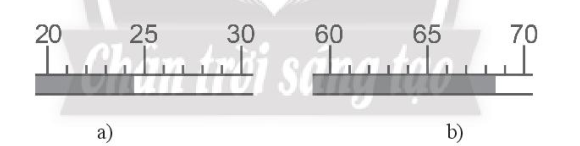
\includegraphics[scale=0.5]{figs/G10Y25B2-2}
		\captionof{figure}{Nhiệt kế: \textit{a) trước; b) sau khi đun dung dịch}}
		\label{fig:3P-1}
	\end{center}
	\loigiai{
		Lấy sai số dụng cụ $\Delta t_\text{dc}=\dfrac{\text{ĐCNN}}{2}=\SI{0.5}{\degree C}$.\\
		Nhiệt độ ban đầu:
		$$t_1=\xsi{24\pm0.5}{\degree C}$$
		Nhiệt độ lúc sau:
		$$t_2=\xsi{68\pm 0.5}{\degree C}$$
		Độ tăng nhiệt độ của dung dịch này:
		$$t=t_2-t_1=\xsi{44.0\pm1.0}{\degree C}.$$
	}
\end{ex}

\begin{ex}
	Hãy xác định số CSCN của các số sau đây: $123,45$; $1,990$; $3,110\cdot 10^{-9}$; $1907,21$; $0,002099$; $12768000$. 
	\loigiai{
		$123,45$ - 5 CSCN; $1,990$ - 4 CSCN; $3,110\cdot10^{-9}$ - 4 CSCN; $1907,21$ - 6 CSCN; $0,002099$ - 4 CSCN; $12768000$ - 5 CSCN.
	}
\end{ex}


\begin{ex}
	Một vật có khối lượng $m$ và thể tích $V$, có khối lượng riêng $\rho$ được xác định bằng công thức $\rho =\dfrac{m}{V}$. Biết sai số tương đối của phép đo $m$ và $V$ lần lượt là $\SI{12}{\percent}$ và $\SI{5}{\percent}$. Hãy xác định sai số tương đối của phép đo $\rho$.
	\loigiai{
		$$\delta \rho=\delta m+\delta V=\SI{12}{\percent}+\SI{5}{\percent}=\SI{17}{\percent}.$$
	}
\end{ex}

\begin{ex}
	Một học sinh muốn xác định gia tốc rơi tự do $g$ bằng cách thả một quả bóng từ độ cao $h$ và dùng đồng hồ để bấm thời gian rơi $t$ của quả bóng. Sau đó, thông qua quá trình tìm hiểu, bạn sử dụng công thức $h=\dfrac{1}{2}g\cdot t^2$ để xác định $g$. Hãy nêu ít nhất 2 giải pháp giúp bạn học sinh đó giảm sai số trong quá trình thực nghiệm để thu được kết quả chính xác nhất.
	\loigiai{
		Một số giải pháp phù hợp: hạn chế sự tác động của lực cản không khí, thả rơi quả bóng ở nhiều độ cao khác nhau, sử dụng đồng hồ có độ nhạy cao, thao tác bấm đồng hồ dứt khoát.
	}
\end{ex}

\begin{ex}
	Bảng ghi thời gian một vật rơi giữa hai điểm cố định:
	\begin{center}
		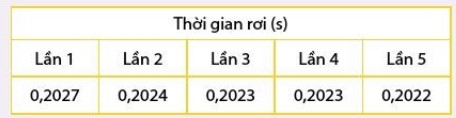
\includegraphics[scale=1]{figs/G10Y25B2-5}
	\end{center}
	\begin{enumerate}[label=\alph*)]
		\item Tính giá trị trung bình của thời gian rơi.
		\item Tìm sai số tuyệt đối trung bình.
	\end{enumerate}
	\loigiai{
		\begin{enumerate}[label=\alph*)]
			\item Giá trị trung bình của thời gian rơi là:
			$$\dfrac{0.2027 + 0.2024+ 0.2023+ 0.2023+ 0.2022}{5} \approx 0.2024$$
			\item Sai số tuyệt đối:
			$$A_1= |0.2024 - 0.2027| = 0.0003.$$
			$$A_2= |0.2024 - 0.2024| = 0.0000.$$
			$$A_3= |0.2024 - 0.2023| = 0.0001.$$
			$$A_4= |0.2024 - 0.2023| = 0.0001.$$
			$$A_5= |0.2024 - 0.2022| = 0.0002.$$
			Sai số tuyệt đối trung bình là: 
			$$\dfrac{0.0003 + 0.0000 + 0.0001 + 0.0001 + 0.0002}{5} = 0.00014.$$
		\end{enumerate}
	}
\end{ex}

\begin{ex}
	Dùng thước kẹp có ĐCNN $\SI{0.1}{mm}$ để đo 5 lần đường kính $d$ và chiều cao $h$ của một trụ thép, cho kết quả như trong bảng sau:
	\begin{center}
		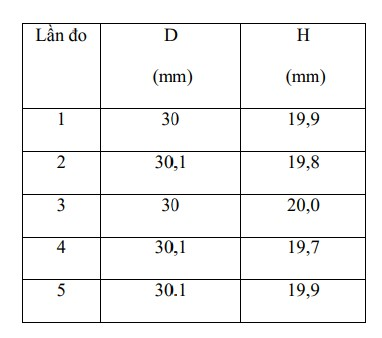
\includegraphics[scale=1]{figs/G10Y25B2-6}
	\end{center}
	Hãy cho biết kết quả phép đo $d, h$ và tính thể tích trụ thép.
	\loigiai{	
		Phép đo $d, h$ là phép đo trực tiếp, giá trị
		trung bình và sai số ngẫu nhiên tính trong
		bảng sau
		\begin{center}
			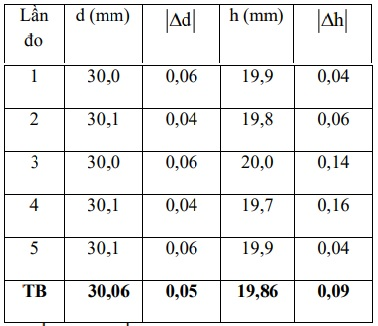
\includegraphics[scale=1]{figs/G10Y25B2-7}
		\end{center}
		Sai số dụng cụ bằng $\SI{0.1}{mm}$. Vậy:
		Sai số phép đo đường kính trụ là:
		$$\Delta d = 0.05 + 0.05 =\SI{0.10}{mm}.$$
		Sai số phép đo chiều cao trụ là:
		$$\Delta h = 0.09 + 0.05 =\SI{0.14}{mm}.$$
		Kết quả: 
		$$d = \xsi{30.06\pm0.10}{\milli\meter}.$$
		$$h = \xsi{19.86\pm0.14}{\milli\meter}.$$
		Thể tích trung bình của khối trụ:
		$$\overline{V} = \dfrac{\pi \overline{d}^2 \overline{h}}{4} =\SI{14094.42}{\cubic\milli\meter}.$$
		Sai số tỉ đối:
		$$\dfrac{\Delta V}{\overline V} = 2 \dfrac{\overline{\Delta d}}{\overline d} + \dfrac{\overline {\Delta h}}{\overline{h}} + \dfrac{\Delta \pi}{\pi} = 0.014 = \SI{1.4}{\percent}.$$
		Sai số tuyệt đối:
		$$\Delta V = \overline{V} \cdot \delta V = \SI{193.13}{\cubic\milli\meter}.$$
		Suy ra:
		$$V = \xsi{14094\pm193}{\cubic\milli\meter}.$$
	}
\end{ex}
\Closesolutionfile{ans}